\documentclass[11pt]{article}

\usepackage[margin=1in]{geometry}
\usepackage[T1]{fontenc}
\usepackage{lmodern}
\usepackage{microtype}
\usepackage{amsmath,amssymb,amsthm,mathtools}
\usepackage{bm}
\usepackage{booktabs}
\usepackage{array}
\usepackage{graphicx}
\usepackage{xcolor}
\usepackage{enumitem}
\usepackage{placeins}
\usepackage[numbers,sort&compress]{natbib}
\usepackage[hidelinks]{hyperref}
\usepackage[nameinlink,noabbrev]{cleveref}

\newtheorem{theorem}{Theorem}[section]
\newtheorem{proposition}[theorem]{Proposition}
\newtheorem{corollary}[theorem]{Corollary}
\newtheorem{lemma}[theorem]{Lemma}
\theoremstyle{definition}
\newtheorem{definition}[theorem]{Definition}
\newtheorem{assumption}[theorem]{Assumption}
\theoremstyle{remark}
\newtheorem{remark}[theorem]{Remark}

\DeclareMathOperator{\supp}{supp}
\DeclareMathOperator{\MMD}{MMD}
\DeclareMathOperator{\vecop}{vec}
\DeclareMathOperator{\id}{id}
\newcommand{\cX}{\mathcal X}
\newcommand{\cY}{\mathcal Y}
\newcommand{\cC}{\mathcal C}
\newcommand{\cS}{\mathcal S}
\newcommand{\cG}{\mathcal G}
\newcommand{\cK}{\mathcal K}
\newcommand{\cB}{\mathcal B}
\newcommand{\bP}{\mathbb P}
\newcommand{\bE}{\mathbb E}
\newcommand{\bR}{\mathbb R}
\newcommand{\bZ}{\mathbb Z}
\newcommand{\indep}{\mathrel{\perp\!\!\!\perp}}
\newcommand{\1}{\mathbf 1}
\newcommand{\given}{\,\middle|\,}
\newcommand{\pending}{\textnormal{\textit{pending}}}

% Empirical values are written by the reproducible analysis into results.tex.
% These defaults keep the manuscript compilable before a run is complete.
\newif\ifresultsavailable
\resultsavailablefalse
\providecommand{\SoftwareCommit}{\pending}
\providecommand{\SoftwareTestsPassed}{\pending}
\providecommand{\SimNullReplicates}{250}
\providecommand{\SimAlternativeReplicates}{750}
\providecommand{\SimReplicatesPerEffect}{250}
\providecommand{\SimBlocks}{8}
\providecommand{\SimPermutationCount}{256}
\providecommand{\SimEffectSizes}{0, 0.35, 0.70, 1.00}
\providecommand{\SimInvariantAuditTrials}{\pending}
\providecommand{\SimInvariantAuditFailures}{\pending}
\providecommand{\SimRawTypeI}{\pending}
\providecommand{\SimRawTypeICI}{\pending}
\providecommand{\SimCanonicalTypeI}{\pending}
\providecommand{\SimCanonicalTypeICI}{\pending}
\providecommand{\SimEulerTypeI}{\pending}
\providecommand{\SimEulerTypeICI}{\pending}
\providecommand{\SimRawPower}{\pending}
\providecommand{\SimCanonicalPower}{\pending}
\providecommand{\SimEulerPower}{\pending}
\providecommand{\SimTableRows}{\multicolumn{6}{c}{\pending}\\}
\providecommand{\RxTreatmentA}{\pending}
\providecommand{\RxTreatmentB}{\pending}
\providecommand{\RxDiscoveryBatches}{12}
\providecommand{\RxConfirmationBatches}{8}
\providecommand{\RxSelectedPairs}{10}
\providecommand{\RxReplicationPairs}{9}
\providecommand{\RxConfirmationBlocks}{8}
\providecommand{\RxPlateAudit}{not yet completed}
\providecommand{\RxManifestHash}{\pending}
\providecommand{\RxPermutationCount}{256}
\providecommand{\RxCanonicalMMD}{\pending}
\providecommand{\RxCanonicalMMDCI}{\pending}
\providecommand{\RxCanonicalP}{\pending}
\providecommand{\RxEulerMMD}{\pending}
\providecommand{\RxEulerMMDCI}{\pending}
\providecommand{\RxEulerP}{\pending}
\providecommand{\RxRawMMD}{\pending}
\providecommand{\RxRawMMDCI}{\pending}
\providecommand{\RxRawP}{\pending}
\providecommand{\RxMomentMMD}{\pending}
\providecommand{\RxMomentMMDCI}{\pending}
\providecommand{\RxMomentP}{\pending}
\providecommand{\RxHolmCanonicalP}{\pending}
\providecommand{\RxHolmEulerP}{\pending}
\providecommand{\RxInvariantAuditTrials}{\pending}
\providecommand{\RxInvariantAuditFailures}{\pending}
\providecommand{\RxBootstrapReplicates}{10000}
\providecommand{\RxNuisanceSeeds}{20}
\providecommand{\RxReplicationSummary}{Secondary-contrast results are populated automatically after the frozen analysis is executed.}
\providecommand{\RxReplicationRows}{\multicolumn{5}{c}{\pending}\\}
\providecommand{\RxAcquisitionNullRows}{\multicolumn{4}{c}{\pending}\\}
\providecommand{\RxApproximateStressRows}{\multicolumn{5}{c}{\pending}\\}
\providecommand{\RxMaxQuotientFeatureError}{\pending}
\providecommand{\RxMaxEulerFeatureError}{\pending}
\providecommand{\RxMaxQuotientStatisticError}{\pending}
\providecommand{\RxMaxQuotientPError}{\pending}
\providecommand{\AbstractSimulationResult}{The frozen simulation has not completed, so no numerical result is reported.}
\providecommand{\AbstractRxResult}{The frozen RxRx1 analysis has not completed, so no numerical result is reported.}
\IfFileExists{results.tex}{% Generated by scripts/build_results_tex.py; do not edit manually.
% source fingerprint: e9f042c387cf
\resultsavailabletrue
\renewcommand{\SoftwareCommit}{source-e9f042c387cf}
\renewcommand{\SoftwareTestsPassed}{45}

\renewcommand{\SimNullReplicates}{250}
\renewcommand{\SimAlternativeReplicates}{750}
\renewcommand{\SimReplicatesPerEffect}{250}
\renewcommand{\SimBlocks}{8}
\renewcommand{\SimPermutationCount}{256}
\renewcommand{\SimEffectSizes}{0, 0.35, 0.7, 1}
\renewcommand{\SimInvariantAuditTrials}{1000}
\renewcommand{\SimInvariantAuditFailures}{0}
\renewcommand{\SimRawTypeI}{1.0000}
\renewcommand{\SimRawTypeICI}{(0.9854, 1.0000)}
\renewcommand{\SimCanonicalTypeI}{0.0520}
\renewcommand{\SimCanonicalTypeICI}{(0.0280, 0.0873)}
\renewcommand{\SimEulerTypeI}{0.0400}
\renewcommand{\SimEulerTypeICI}{(0.0193, 0.0723)}
\renewcommand{\SimRawPower}{1.0000}
\renewcommand{\SimCanonicalPower}{0.9920}
\renewcommand{\SimEulerPower}{1.0000}
\renewcommand{\SimTableRows}{%
Exact quotient & 0.0520 (0.0280, 0.0873) & 0.1400 & 0.8480 & 0.9920 & 256\\
Raw pixels & 1.0000 (0.9854, 1.0000) & 1.0000 & 1.0000 & 1.0000 & 256\\
Moment registration & 0.0560 (0.0310, 0.0922) & 0.5400 & 0.9960 & 1.0000 & 256\\
Finite Euler signature & 0.0400 (0.0193, 0.0723) & 0.1840 & 1.0000 & 1.0000 & 256\\
}

\renewcommand{\RxTreatmentA}{\texttt{s38230}}
\renewcommand{\RxTreatmentB}{\texttt{s37149}}
\renewcommand{\RxDiscoveryBatches}{12}
\renewcommand{\RxConfirmationBatches}{8}
\renewcommand{\RxSelectedPairs}{10}
\renewcommand{\RxReplicationPairs}{9}
\renewcommand{\RxConfirmationBlocks}{8}
\renewcommand{\RxPlateAudit}{passed for all frozen pairs and blocks}
\renewcommand{\RxManifestHash}{b6f350ca96fb9e7a6271845dd6e432ed9dca556144a1a332d8f5af168642b968}
\renewcommand{\RxPermutationCount}{256}
\renewcommand{\RxCanonicalMMD}{0.0036}
\renewcommand{\RxCanonicalMMDCI}{(0.0415, 0.3505)}
\renewcommand{\RxCanonicalP}{0.0078}
\renewcommand{\RxEulerMMD}{0.7535}
\renewcommand{\RxEulerMMDCI}{(0.5582, 1.2290)}
\renewcommand{\RxEulerP}{0.0078}
\renewcommand{\RxRawMMD}{0.1664}
\renewcommand{\RxRawMMDCI}{(0.2008, 0.5021)}
\renewcommand{\RxRawP}{0.0078}
\renewcommand{\RxMomentMMD}{-0.0065}
\renewcommand{\RxMomentMMDCI}{(0.0297, 0.3431)}
\renewcommand{\RxMomentP}{0.2109}
\renewcommand{\RxHolmCanonicalP}{0.0703}
\renewcommand{\RxHolmEulerP}{0.0703}
\renewcommand{\RxInvariantAuditTrials}{6400}
\renewcommand{\RxInvariantAuditFailures}{0}
\renewcommand{\RxBootstrapReplicates}{10000}
\renewcommand{\RxNuisanceSeeds}{20}
\renewcommand{\RxReplicationRows}{%
1 & \texttt{s21474} versus \texttt{s21486} & 0.0040 & 0.0859 & 0.1719\\
2 & \texttt{s29342} versus \texttt{s28343} & 0.0045 & 0.0156 & 0.0703\\
3 & \texttt{s18592} versus \texttt{s18763} & 0.1266 & 0.0078 & 0.0703\\
4 & \texttt{s20782} versus \texttt{s21523} & 0.0031 & 0.0078 & 0.0703\\
5 & \texttt{s20401} versus \texttt{s19178} & 0.0228 & 0.0156 & 0.0703\\
6 & \texttt{s29371} versus \texttt{s28116} & 0.0063 & 0.0078 & 0.0703\\
7 & \texttt{s17831} versus \texttt{s20468} & 0.0486 & 0.0078 & 0.0703\\
8 & \texttt{s37483} versus \texttt{s224918} & -0.0107 & 0.1562 & 0.1719\\
9 & \texttt{s37712} versus \texttt{s224940} & 0.0761 & 0.0078 & 0.0703\\
}
\renewcommand{\RxReplicationSummary}{0 of the nine frozen secondary contrasts remained significant after Holm adjustment.}
\renewcommand{\RxAcquisitionNullRows}{%
Exact quotient & 200 & 0 & 0.0000 (0.0000, 0.0183)\\
Finite Euler signature & 200 & 0 & 0.0000 (0.0000, 0.0183)\\
Moment registration & 200 & 0 & 0.0000 (0.0000, 0.0183)\\
Raw pixels & 200 & 200 & 1.0000 (0.9817, 1.0000)\\
\multicolumn{4}{p{0.92\linewidth}}{\footnotesize Parentheses give exact binomial Clopper--Pearson intervals as descriptive summaries only; pair--seed tests share biological blocks and are not independent Bernoulli trials.}\\
}
\renewcommand{\RxApproximateStressRows}{%
Rotation \(5^\circ\) & Exact quotient & 0.8432 & 0.0012 & 0.0000\\
Rotation \(5^\circ\) & Finite Euler signature & 0.0779 & 0.0860 & 0.0000\\
Rotation \(5^\circ\) & Moment registration & 0.7295 & 0.0014 & 0.0234\\
Rotation \(5^\circ\) & Raw pixels & 0.6540 & 0.0013 & 0.0000\\
Rotation \(10^\circ\) & Exact quotient & 0.8967 & 0.0022 & 0.0000\\
Rotation \(10^\circ\) & Finite Euler signature & 0.0827 & 0.0530 & 0.0000\\
Rotation \(10^\circ\) & Moment registration & 0.8124 & 0.0021 & 0.1250\\
Rotation \(10^\circ\) & Raw pixels & 0.8038 & 0.0012 & 0.0000\\
Rotation \(20^\circ\) & Exact quotient & 0.9715 & 0.0005 & 0.0000\\
Rotation \(20^\circ\) & Finite Euler signature & 0.1076 & 0.0898 & 0.0000\\
Rotation \(20^\circ\) & Moment registration & 0.8662 & 0.0009 & 0.0469\\
Rotation \(20^\circ\) & Raw pixels & 0.8802 & 0.0014 & 0.0000\\
Two-pixel support crop & Exact quotient & 0.8253 & 0.0026 & 0.0000\\
Two-pixel support crop & Finite Euler signature & 0.1478 & 0.0164 & 0.0000\\
Two-pixel support crop & Moment registration & 0.6857 & 0.0203 & 0.2031\\
Two-pixel support crop & Raw pixels & 0.3523 & 0.0001 & 0.0000\\
Within-support Gaussian noise & Exact quotient & 0.5949 & 0.0007 & 0.0000\\
Within-support Gaussian noise & Finite Euler signature & 0.0618 & 0.0244 & 0.0000\\
Within-support Gaussian noise & Moment registration & 0.3870 & 0.0067 & 0.1328\\
Within-support Gaussian noise & Raw pixels & 0.1775 & 0.0006 & 0.0000\\
}
\renewcommand{\RxMaxQuotientFeatureError}{0.0000}
\renewcommand{\RxMaxEulerFeatureError}{0.0000}
\renewcommand{\RxMaxQuotientStatisticError}{0.0000}
\renewcommand{\RxMaxQuotientPError}{0.0000}

\renewcommand{\AbstractSimulationResult}{Under the sharp null, the maximal-invariant test rejected in 0.0520 of replicates; at effect strength 1.0000, its power was 0.9920.}
\renewcommand{\AbstractRxResult}{For the primary RxRx1 contrast, the canonical quotient comparison gave an enumerated paired-swap \(p\)-value of 0.0078.}
}{}
\newif\ifextensionsavailable
\extensionsavailablefalse
\newcommand{\RxSensitivityRows}{\multicolumn{2}{c}{\pending}\\}
\newcommand{\RxSensitivityCritical}{\pending}
\newcommand{\RxSensitivityCriticalP}{\pending}
\newcommand{\RxExtensionExactP}{\pending}
\newcommand{\RxPersistenceSites}{\pending}
\newcommand{\RxPersistenceInvariantChecks}{\pending}
\newcommand{\RxPersistenceStabilityChecks}{\pending}
\newcommand{\RxPersistenceKernelChecks}{\pending}
\newcommand{\RxPersistenceMaxExactBottleneck}{\pending}
\newcommand{\RxPersistenceMaxPerturbedBottleneck}{\pending}
\newcommand{\RxPersistenceMaxSupNorm}{\pending}
\newcommand{\RxExtensionAuditHash}{\pending}
\IfFileExists{extension_results.tex}{% Generated by scripts/build_extension_results_tex.py; do not hand edit.
\extensionsavailabletrue
\renewcommand{\RxSensitivityRows}{1.00 & 0.007812 \\
1.10 & 0.008311 \\
1.25 & 0.010597 \\
1.50 & 0.017452 \\
2.00 & 0.039171 \\
3.00 & 0.100128 \\
5.00 & 0.232569 \\}
\renewcommand{\RxSensitivityCritical}{2.199995}
\renewcommand{\RxSensitivityCriticalP}{0.050000}
\renewcommand{\RxExtensionExactP}{0.0078125}
\renewcommand{\RxPersistenceSites}{32}
\renewcommand{\RxPersistenceInvariantChecks}{32}
\renewcommand{\RxPersistenceStabilityChecks}{32}
\renewcommand{\RxPersistenceKernelChecks}{32}
\renewcommand{\RxPersistenceMaxExactBottleneck}{0.000000}
\renewcommand{\RxPersistenceMaxPerturbedBottleneck}{0.003918}
\renewcommand{\RxPersistenceMaxSupNorm}{0.003920}
\renewcommand{\RxExtensionAuditHash}{7928f075dd02630e2c735a89bbd64e8a76f8b9191b2785cfe8de6542462c0882}
}{}

\title{Causal Inference for Group-Contaminated Structured Outcomes:
Quotient Identification and Exact Randomization Inference}
\author{Author names omitted for blinded review}
\date{}

\begin{document}
\maketitle

\begin{abstract}
Structured potential outcomes such as microscopy images can be recorded after an
unknown, unit-specific acquisition transformation.  If that transformation may
depend on treatment, covariates, or the intrinsic outcome, analyses in raw
coordinates can confound a treatment contrast with acquisition geometry.  We
formulate this problem as a measurable group action and characterize exactly
which intrinsic targets remain observable: a target admits a decoder under
unrestricted contamination if and only if it is constant on group orbits.  When
a Borel maximal invariant exists, its complete interventional distribution is
identified under consistency, positivity, and exchangeability for that
invariant.  For finite-support multichannel lattice images, we construct an
explicit maximal invariant under integer translations and quarter-turn
rotations, and combine its Gaussian kernel with a complete paired-swap test of
the Fisher sharp null for quotient outcomes.  Conditional finite-sample
validity requires well-defined reagent conditions, no cross-well interference,
swap-invariant block retention, and uniform within-plate pair assignments.  We evaluate the
method in controlled simulations and in a discovery--confirmation study of
\(\RxSelectedPairs\) disjoint siRNA pairs using six-channel RxRx1 HUVEC
microscopy wells.  The confirmation images are subjected to treatment- and
outcome-dependent lattice rigid motions whose realized parameters are excluded
from the estimators; inference uses only the transformed images and treatment
labels from the reported within-plate randomization.
\AbstractSimulationResult\ \AbstractRxResult
\end{abstract}

\noindent\textbf{Keywords:} causal inference; group action; maximal invariant;
microscopy image; quotient space; randomization test; structured outcome

\section{Introduction}

Many experimental outcomes are structured objects rather than scalars.  An
image, shape, network, or function may be represented in a coordinate system
that varies from unit to unit.  In microscopy, for example, translation or
orientation can arise from acquisition and preprocessing rather than from the
biological intervention.  We study the observation model
\begin{equation}\label{eq:observation-model}
  X=\Gamma\cdot Y(A),
\end{equation}
where \(A\) is treatment, \(Y(a)\) is the intrinsic structured potential outcome,
and \(\Gamma\) is an unobserved transformation.  Crucially, no independence
between \(\Gamma\) and \(A\), covariates, or potential outcomes is imposed.
Thus, averaging over a posited nuisance distribution is neither required nor
available.

The central issue is not whether a representation is predictive, but which
causal target is determined by \eqref{eq:observation-model}.  We first prove a
sharp observability theorem: exact recovery under every admissible
transformation is equivalent to orbit invariance.  We then separate
observability from causal identification.  A maximal invariant records the
entire orbit and therefore represents the richest observable target.  Under
standard target-specific causal assumptions, the \(g\)-formula identifies its
full interventional law.  This distinction is important: invariance removes the
acquisition nuisance, whereas exchangeability or randomization connects factual
and counterfactual distributions.

Our empirical construction concerns two-site, six-channel lattice images.  The
group is the lattice rigid-motion group
\(\bZ^2\rtimes C_4\), acting separately on the two sites of a well.  We
translate each rotated support to a fixed origin and retain the
lexicographically least shape-aware serialization among the four rotations.
The resulting deterministic map is a Borel maximal invariant even though the
translation group is noncompact.  A Gaussian kernel pulled back through this
map is positive definite, invariant, and characteristic for probability laws
on the quotient.  This supports a kernel two-sample statistic and an exact test
of the Fisher sharp null by within-block randomization.

\subsection{Relation to prior work}

Causal methods for non-Euclidean outcomes commonly take the outcome as an
observed element of a specified metric space.  Geodesic causal inference uses
Fr\'echet regression and geodesic treatment contrasts
\citep{kurisu2024geodesic}; recent doubly robust work embeds random-object
outcomes into a known Hilbert space \citep{bhattacharjee2025doubly}.  These
frameworks address rich outcome geometry but do not include a latent,
unit-specific group action in the observation equation.  Causal analysis on a
quotient space is itself not new: \citet{shin2024absolute} include an
application in Kendall shape space, which removes translation, scale, and
rotation for pre-corresponded landmarks.  For functional outcomes,
\citet{raykov2025kernel} perform registration before kernel estimation.  Our
object is different and complementary: full-law identification for the
observable orbit and exact Fisher-sharp-null testing on that orbit when the
recorded object is contaminated by an unknown group element.

Topological transforms provide useful structured summaries.  The persistent
homology transform and Euler characteristic transform can be injective on
specified tame shape classes when the full directional transform is available
\citep{turner2014persistent,curry2022directions}.  In the experiment below, a
fixed, finite directional Euler vector is used only as a prespecified secondary
signature after exact orbit canonicalization.  All full-law claims in this
article concern the maximal invariant, not that finite vector.

\citet{kim2026topological} propose estimands based on power-weighted persistence
silhouettes, while \citet{saki2026beyond} formulate conditional
persistence-summary estimands under persistent-homology ignorability.  These
works target chosen summaries of outcome laws; our finite Euler vector is
secondary, whereas the full-law identification result below concerns a maximal
orbit code under a latent group action.

The RxRx1 collection provides high-dimensional, replicated Cell Painting
images with substantial experimental variation
\citep{sypetkowski2023rxrx1,rxrx1website}.  Its reported plate-level randomization and
multiple HUVEC experiments permit row-excluded confirmation tests, provided that
the two siRNAs in each contrast belong to the same plate randomization set.  We
enforce that condition before examining confirmation outcomes.

\section{Observation, quotient targets, and identification}

\subsection{Measurable group contamination}

Let \(\cY\), \(\cC\), \(\cS\), and \(\cG\) be standard Borel spaces.  Assume
that \(\cG\) is a measurable group, meaning that multiplication and inversion
are Borel, and that it acts on \(\cY\) by a jointly Borel map
\((g,y)\mapsto g\cdot y\), satisfying \(e\cdot y=y\) and
\(g\cdot(h\cdot y)=(gh)\cdot y\).  The orbit of \(y\) is
\([y]_{\cG}=\{g\cdot y:g\in\cG\}\).  A Borel map
\(\tau:\cY\to\cS\) is \(\cG\)-invariant if
\(\tau(g\cdot y)=\tau(y)\) for all \(g,y\).

For treatment values \(a\) in a finite set \(\mathcal A\), let \(Y(a)\) be the
intrinsic potential outcome.  We observe \(O=(C,A,X)\), with
\[
  X=\Gamma\cdot Y(A),
\]
where \(\Gamma\) is an unobserved, possibly stochastic element of \(\cG\).
The conditional distribution of \(\Gamma\) is unrestricted.

\begin{theorem}[Sharp observability]\label{thm:sharp}
For a Borel target \(\tau:\cY\to\cS\), the following statements are equivalent.
\begin{enumerate}[label=(\roman*)]
  \item There is a Borel decoder \(D:\cY\to\cS\) such that
  \(D(g\cdot y)=\tau(y)\) for every \(g\in\cG\) and \(y\in\cY\).
  \item The target \(\tau\) is \(\cG\)-invariant.
\end{enumerate}
\end{theorem}

\begin{proof}
If \(\tau\) is invariant, take \(D=\tau\).  Then
\(D(g\cdot y)=\tau(g\cdot y)=\tau(y)\).  Conversely, suppose (i) holds.
Using the identity element gives \(D(z)=\tau(z)\) for every \(z\in\cY\).
For arbitrary \(g,y\), apply this equality at \(z=g\cdot y\) and then use (i):
\[
  \tau(g\cdot y)=D(g\cdot y)=\tau(y).
\]
Hence \(\tau\) is invariant.
\end{proof}

\begin{corollary}[Nonidentifiability outside the quotient]\label{cor:nonid}
If \(\tau\) is not invariant, there are two data-generating processes satisfying
\eqref{eq:observation-model} that induce the same observed law but different
laws of \(\tau\{Y(a)\}\), for any fixed \(a\).
\end{corollary}

\begin{proof}
Choose \(y\in\cY\) and \(g\in\cG\) such that
\(\tau(g\cdot y)\ne\tau(y)\), and take \(A=a\) almost surely.  In the first process set
\(Y(a)=y\) and \(\Gamma=g\) almost surely; in the second set
\(Y(a)=g\cdot y\) and \(\Gamma=e\) almost surely.  Hold all other observed
variables fixed and identical.  Both processes yield \(X=g\cdot y\) almost
surely, but their target values are \(\tau(y)\) and \(\tau(g\cdot y)\).
\end{proof}

The full-support observation model is important.  If acquisition includes a
lossy operation such as a field-of-view crop, orbit invariance alone is no
longer sufficient.  The next result gives the sharp replacement.

\begin{theorem}[Sharp observability after partial acquisition]
\label{thm:partial-observation}
Let \(\cG,\cY,\cX,\cS\) be standard Borel spaces, let \(\cG\) act jointly
Borelly on \(\cY\), and let \(\Pi:\cY\to\cX\) be a Borel observation
operator.  Define \(\Phi:\cG\times\cY\to\cX\) by
\[
  \Phi(g,y)=\Pi(g\cdot y).
\]
For a Borel target \(\tau:\cY\to\cS\), the following are equivalent.
\begin{enumerate}[label=(\roman*)]
  \item There is a Borel decoder \(D:\cX\to\cS\) such that
  \[
    D\{\Pi(g\cdot y)\}=\tau(y)
    \quad\text{for every }g\in\cG\text{ and }y\in\cY.
  \]
  \item For every \(g,h\in\cG\) and \(y,z\in\cY\),
  \[
    \Pi(g\cdot y)=\Pi(h\cdot z)
    \quad\Longrightarrow\quad
    \tau(y)=\tau(z).
  \]
\end{enumerate}
\end{theorem}

\begin{proof}
Condition (i) immediately implies (ii).  Conversely, define the Borel map
\(\widetilde\tau:\cG\times\cY\to\cS\) by
\(\widetilde\tau(g,y)=\tau(y)\).  Condition (ii) says precisely that
\(\widetilde\tau\) is constant on every fiber of \(\Phi\).

For a Borel set \(B\subseteq\cS\), put
\(A=\widetilde\tau^{-1}(B)\).  The analytic sets \(\Phi(A)\) and
\(\Phi\{(\cG\times\cY)\setminus A\}\) are disjoint.  The Lusin separation
theorem therefore supplies a Borel set \(E_B\subseteq\cX\) such that
\[
  \Phi(A)\subseteq E_B,
  \qquad
  \Phi\{(\cG\times\cY)\setminus A\}
  \subseteq\cX\setminus E_B.
\]
It follows that \(A=\Phi^{-1}(E_B)\), so \(\widetilde\tau\) is
\(\sigma(\Phi)\)-measurable.  The measurable factorization lemma for standard
Borel codomains gives a Borel \(D:\cX\to\cS\) satisfying
\(\widetilde\tau=D\circ\Phi\), which is (i).
\end{proof}

\begin{corollary}[Partial-observation nonidentifiability]
\label{cor:partial-nonid}
If \(\Pi(g\cdot y)=\Pi(h\cdot z)\) for some \(g,h,y,z\), but
\(\tau(y)\ne\tau(z)\), then two data-generating processes can induce the same
observed law and different laws of \(\tau\{Y(a)\}\).
\end{corollary}

\begin{proof}
Take \(A=a\) almost surely.  In the first process set \(Y(a)=y\) and
\(\Gamma=g\); in the second set \(Y(a)=z\) and \(\Gamma=h\).  Hold every
other observed variable fixed and identical.  The recorded value is the same
in both processes by hypothesis, while the target values differ.
\end{proof}

\subsection{Maximal invariants}

\begin{definition}\label{def:maximal}
A Borel map \(M:\cY\to\cS\) is a \emph{maximal invariant} if
\[
  M(y)=M(z)\quad\Longleftrightarrow\quad z=g\cdot y
  \text{ for some }g\in\cG .
\]
\end{definition}

Thus \(M\) labels orbits without distinguishing points within an orbit.  The
next theorem makes precise the sense in which it contains every observable
target.  The standard Borel hypotheses are substantive; without them, a
set-theoretic quotient need not admit the required measurable factorization.
This is the measurable analogue of the role played by maximal invariants in
classical invariant decision problems \citep{eaton1989group}.

\begin{theorem}[Borel factorization through a maximal invariant]
\label{thm:factorization}
Let \(\cY,\cS,\mathcal T\) be standard Borel spaces, and let
\(M:\cY\to\cS\) be a Borel maximal invariant.  Every Borel invariant
\(h:\cY\to\mathcal T\) has a Borel factorization
\[
  h=\bar h\circ M
\]
for some Borel \(\bar h:\cS\to\mathcal T\).  The restriction of
\(\bar h\) to \(M(\cY)\) is unique.
\end{theorem}

\begin{proof}
Fix a Borel set \(B\subseteq\mathcal T\) and put
\(A=h^{-1}(B)\).  Invariance of \(h\) and maximality of \(M\) imply that
\(A\) is saturated for the fibers of \(M\).  Therefore the analytic sets
\(M(A)\) and \(M(\cY\setminus A)\) are disjoint.  By the Lusin separation
theorem for standard Borel spaces \citep[Theorem 14.7]{kechris1995classical},
there is a Borel set \(D_B\subseteq\cS\) such that
\[
  M(A)\subseteq D_B,\qquad
  M(\cY\setminus A)\subseteq\cS\setminus D_B.
\]
Consequently \(A=M^{-1}(D_B)\), so every inverse image under \(h\) is in
\(\sigma(M)\).  Hence \(h\) is \(\sigma(M)\)-measurable.  The measurable
factorization lemma for standard Borel codomains
\citep[Lemma 1.13]{kallenberg2021foundations} yields a Borel map
\(\bar h\) such that \(h=\bar h\circ M\).  If two such maps differ at a
point \(M(y)\), their compositions differ at \(y\), proving uniqueness on
\(M(\cY)\).
\end{proof}

Existence of a Borel maximal invariant is not automatic for an arbitrary
measurable action.  Compact continuous actions give an important sufficient
condition.

\begin{proposition}[Orbit code for a compact action]\label{prop:compact}
Let \(\cG\) be a compact metrizable group acting continuously on a Polish space
\(\cY\).  Let \(\cK(\cY)\) be the hyperspace of nonempty compact subsets of
\(\cY\), equipped with its Vietoris Borel structure.  Then
\[
  M_{\mathrm{orb}}(y)=\cG\cdot y
\]
is a Borel maximal invariant taking values in the standard Borel space
\(\cK(\cY)\).
\end{proposition}

\begin{proof}
The orbit is compact because it is the continuous image of compact \(\cG\).
For an open set \(U\subseteq\cY\),
\[
\begin{split}
 \{y:M_{\mathrm{orb}}(y)\cap U\ne\varnothing\}
   &=\bigcup_{g\in\cG}g^{-1}U,\\
 \{y:M_{\mathrm{orb}}(y)\subseteq U\}
   &=\cY\setminus\bigcup_{g\in\cG}g^{-1}(\cY\setminus U).
\end{split}
\]
The first set is open.  To prove that the second is open, fix \(y\) with
\(\cG\cdot y\subset U\).  For each \(g\in\cG\), joint continuity supplies
neighborhoods \(N_g\) of \(g\) and \(V_g\) of \(y\) such that
\(N_g\cdot V_g\subset U\).  Compactness of \(\cG\) gives
\(g_1,\ldots,g_r\) with \(\cG=\bigcup_{i=1}^rN_{g_i}\).  The neighborhood
\(V=\bigcap_{i=1}^rV_{g_i}\) of \(y\) then satisfies
\(\cG\cdot V\subset U\).  Hence the second set is open.  These two classes
generate the Vietoris topology, so \(M_{\mathrm{orb}}\) is continuous and in
particular Borel.  Finally,
\(M_{\mathrm{orb}}(y)=M_{\mathrm{orb}}(z)\) holds exactly when
\(z\in\cG\cdot y\), establishing maximality.
\end{proof}

\begin{corollary}[Continuous rotations]\label{cor:continuous-rotations}
Let \(\operatorname{SO}(2)\) act continuously on a Polish space \(\cY\).  Then
\[
  M_{\mathrm{rot}}(y)
  =\{R_\theta\cdot y:\theta\in[0,2\pi)\}
\]
is a Borel maximal invariant with values in \(\cK(\cY)\).
\end{corollary}

\begin{proof}
The group \(\operatorname{SO}(2)\) is compact and metrizable, so
\cref{prop:compact} applies.
\end{proof}

This corollary is an orbit-valued existence result.  It does not construct a
finite-dimensional canonical representative for continuously rotated raster
images, and common interpolation rules on a fixed lattice need not define an
exact group action.  The Euclidean rigid-motion group
\(\operatorname{SE}(2)=\bR^2\rtimes\operatorname{SO}(2)\) is noncompact, so
\cref{prop:compact} gives no conclusion for that larger group.  Noncompactness
by itself is not an impossibility result, as the explicit integer-translation
construction in \cref{sec:lattice} demonstrates.

\begin{proposition}[Canonical maximal invariant for a finite group]
\label{prop:finite-canonical}
Let a finite group \(H=\{h_1,\ldots,h_m\}\) act by Borel maps on a standard
Borel space \(\cY\), and let \(\nu:\cY\to[0,1]\) be a Borel injection.  Define
\[
 j^\star(y)=\min\arg\min_{1\le j\le m}\nu(h_j\cdot y),
 \qquad c_H(y)=h_{j^\star(y)}\cdot y.
\]
Then \(c_H\) is a Borel maximal invariant for the \(H\)-action.
\end{proposition}

\begin{proof}
Put \(f_j(y)=\nu(h_j\cdot y)\).  Each \(f_j\) is Borel, and
\[
 \{y:j^\star(y)=j\}
 =
 \bigcap_{k<j}\{y:f_j(y)<f_k(y)\}
 \cap
 \bigcap_{k>j}\{y:f_j(y)\le f_k(y)\}.
\]
Thus \(j^\star\), and hence \(c_H\), is Borel.  Let
\(\mathcal O_y=\{h\cdot y:h\in H\}\) be the finite set of distinct orbit
points.  Injectivity of \(\nu\) makes the \(\nu\)-values of distinct points in
\(\mathcal O_y\) distinct.  Therefore the finite set \(\nu(\mathcal O_y)\)
has a unique least value, attained by one orbit point \(u_y\).  Several
minimizing indices can occur only when they represent this same point, as may
happen under a nontrivial stabilizer.  Consequently \(c_H(y)=u_y\).

If \(z=h\cdot y\), then \(\mathcal O_z=\mathcal O_y\), so
\(c_H(z)=u_z=u_y=c_H(y)\).  Conversely, if \(c_H(y)=c_H(z)\), this common
point belongs to both orbits.  Two group orbits that intersect are equal, and
hence \(z=h\cdot y\) for some \(h\in H\).
\end{proof}

\subsection{Identification of the interventional quotient law}

Let \(Q(a)=M\{Y(a)\}\).  Invariance gives the observed quotient outcome
\begin{equation}\label{eq:q-observed}
  Q=M(X)=M\{\Gamma\cdot Y(A)\}=M\{Y(A)\}=Q(A)
\end{equation}
without any assumption on \(\Gamma\).

\begin{assumption}[Quotient causal conditions]\label{ass:causal}
For each \(a\in\mathcal A\):
\begin{enumerate}[label=(\alph*)]
  \item quotient consistency holds as in \eqref{eq:q-observed};
  \item \(Q(a)\indep A\mid C\);
  \item \(\bP(A=a\mid C)>0\) almost surely.
\end{enumerate}
\end{assumption}

\begin{theorem}[Identification of the full quotient law]\label{thm:gformula}
Under \cref{ass:causal}, for every Borel \(B\subseteq\cS\),
\begin{equation}\label{eq:gformula}
 \bP\{Q(a)\in B\}
 =
 \int \bP(Q\in B\mid A=a,C=c)\,dP_C(c).
\end{equation}
Consequently, the entire probability law of the maximal invariant under
intervention \(a\) is identified.
\end{theorem}

\begin{proof}
Standard Borel spaces admit regular conditional distributions.  Iterated
expectation, conditional exchangeability, positivity, and consistency give
\[
\begin{aligned}
\bP\{Q(a)\in B\}
 &=\int \bP\{Q(a)\in B\mid C=c\}\,dP_C(c)\\
 &=\int \bP\{Q(a)\in B\mid A=a,C=c\}\,dP_C(c)\\
 &=\int \bP(Q\in B\mid A=a,C=c)\,dP_C(c).
\end{aligned}
\]
The equality for every Borel \(B\) determines the probability measure on
\(\cS\).
\end{proof}

By \cref{thm:factorization}, the interventional law of any Borel invariant
target \(h\{Y(a)\}\) is then the pushforward of the identified law in
\eqref{eq:gformula} through \(\bar h\).  This is a property of maximality, not
an assertion that an arbitrary lower-dimensional invariant summary is
maximal.  The argument is the ordinary adjustment formula applied to a
quotient-valued potential outcome \citep{rubin1974estimating,
rosenbaum1983central,robins1986new}.

For conditional mean effects, a scalar target must first be specified on the
quotient; an object-valued outcome does not itself admit subtraction.

\begin{corollary}[Conditional effects of scalar invariant functionals]
\label{cor:invariant-cate}
Let \(A\in\{0,1\}\), suppose \cref{ass:causal} holds, and let
\(h:\cS\to\bR\) be Borel with
\(\bE|h\{Q(a)\}|<\infty\) for \(a=0,1\).  Then, for \(P_C\)-almost every
\(c\),
\begin{equation}\label{eq:invariant-cate}
 \tau_h(c)
 :=
 \bE\!\left[h\{Q(1)\}-h\{Q(0)\}\mid C=c\right]
 =
 \bE\{h(Q)\mid A=1,C=c\}
 -
 \bE\{h(Q)\mid A=0,C=c\}.
\end{equation}
\end{corollary}

\begin{proof}
Conditional exchangeability, positivity, and consistency imply, for
\(a=0,1\),
\[
  \bE[h\{Q(a)\}\mid C=c]
  =\bE\{h(Q)\mid A=a,C=c\}
\]
for \(P_C\)-almost every \(c\).  Subtracting the two equalities proves
\eqref{eq:invariant-cate}.
\end{proof}

By \cref{thm:factorization}, every integrable scalar Borel invariant of the
intrinsic outcome can be written in this form.  The corollary identifies the
target; it does not by itself supply a statistically adequate heterogeneous-
effect estimator for a small experiment.

\section{A maximal invariant for lattice microscopy images}
\label{sec:lattice}

\subsection{The lattice rigid-motion action}

Fix \(L<\infty\).  Let \(\cX_{q,L}\) be the space of functions
\[
 x:\bZ^2\longrightarrow\{0,\ldots,255\}^{q},
\]
whose nonempty support bounding box has at most \(L\) rows and \(L\) columns,
together with the identically zero image, equipped with its standard Borel
structure.  This countable space represents a
\(q\)-channel 8-bit image on the full lattice; values outside the finite
support are zero.  The fixed support bound is preserved by lattice translations
and quarter turns and permits an injective embedding of every normalized
representative into one \(q\times L\times L\) canvas.
Let \(C_4=\{0,1,2,3\}\) index counterclockwise rotations
\(R_r\) by \(r\pi/2\).  The semidirect product
\(\cG_{\mathrm{rig}}=\bZ^2\rtimes C_4\) has multiplication
\[
 (t,r)(u,s)=(t+R_r u,\ r+s\bmod 4)
\]
and action
\begin{equation}\label{eq:lattice-action}
 \{(t,r)\cdot x\}(v)=x\{R_r^{-1}(v-t)\},\qquad v\in\bZ^2.
\end{equation}

For nonzero \(x\), let
\[
 b(x)=\left(\min_{v\in\supp(x)}v_1,\ 
            \min_{v\in\supp(x)}v_2\right)
\]
be the lower corner of its support bounding box, and define
\[
 N(x)=(-b(x),0)\cdot x.
\]
For the zero image, set \(N(0)=0\), give it the one-by-one all-zero
serialization, and set \(c(0)=0\).
The ordering key
\(\kappa\{N(x)\}=(h(x),w(x),\operatorname{bytes}\{N(x)\})\) contains the
integer bounding-box dimensions followed by all \(q\)-channel byte values in a
fixed lattice and channel order; keys are compared lexicographically.
Including the dimensions makes the code injective for nonsquare arrays and
their rotations.  For each \(r\in C_4\), form
\[
  x_r=N\{(0,r)\cdot x\},
\]
and let
\begin{equation}\label{eq:canonical}
  c(x)=x_{r^\star},\qquad
  r^\star=\min\arg\min_{r\in C_4}\kappa(x_r),
\end{equation}
where the outer minimum fixes a deterministic index in the event of a
stabilizer.

\begin{theorem}[Lattice rigid-motion canonicalization]\label{thm:lattice}
The map \(c:\cX_{q,L}\to\cX_{q,L}\) in \eqref{eq:canonical} is Borel and is a maximal
invariant for the action of \(\bZ^2\rtimes C_4\):
\[
 c(x)=c(y)\quad\Longleftrightarrow\quad
 y=(t,r)\cdot x\ \text{for some }(t,r)\in\bZ^2\rtimes C_4 .
\]
\end{theorem}

\begin{proof}
The zero image is fixed by the entire group and is the only image whose orbit
contains zero, so the stated equivalence holds whenever \(x=0\) or \(y=0\).
It remains to consider two nonzero images.  All coordinate permutations,
support bounds, finite serializations, and comparisons in
\eqref{eq:canonical} are Borel; a minimum over four Borel maps is Borel.
Translation normalization satisfies
\begin{equation}\label{eq:normalization-shift}
 N\{(t,0)\cdot z\}=N(z),
\end{equation}
because \(b\{(t,0)\cdot z\}=b(z)+t\).

Suppose \(y=(t,s)\cdot x\).  For each \(r\in C_4\), the group law and
\eqref{eq:normalization-shift} give
\[
 N\{(0,r)\cdot y\}
 =N\{(R_rt,r+s)\cdot x\}
 =N\{(0,r+s)\cdot x\}.
\]
As \(r\) ranges over \(C_4\), so does \(r+s\).  The four normalized candidate
sets for \(x\) and \(y\) are therefore equal, so \(c(y)=c(x)\).

Conversely, suppose \(c(x)=c(y)=z\).  For some \(r,s\in C_4\) and
\(u,v\in\bZ^2\),
\[
 z=(u,r)\cdot x=(v,s)\cdot y.
\]
Applying the inverse of \((v,s)\) yields
\[
 y=(v,s)^{-1}(u,r)\cdot x,
\]
which is an element of the same \(\bZ^2\rtimes C_4\) orbit.  This proves both
directions of maximality.
\end{proof}

An RxRx1 well has two labeled sites.  With separate site-specific
acquisition motions, the group is
\(\cG_{\mathrm{well}}=\cG_{\mathrm{rig}}\times\cG_{\mathrm{rig}}\), and
\begin{equation}\label{eq:well-code}
  C(x_1,x_2)=\bigl(c(x_1),c(x_2)\bigr).
\end{equation}
Componentwise application of \cref{thm:lattice} shows that \(C\) is maximal for
the product action.  The construction uses a deterministic cross-section; no
probability measure on the noncompact translation group is introduced.

\subsection{Invariant kernels and a finite Euler signature}

Fix a storage bound \(L_0\ge L\).  Let
\(\psi\{C(w)\}\in\bR^{2qL_0^2}\) concatenate the two canonical support crops
after placing each crop at the upper-left corner of an \(L_0\times L_0\) zero
canvas.  Because each crop is its minimal nonzero support bounding box, this
fixed-dimensional Borel embedding is injective on canonical representatives.
For \(\sigma>0\), define
\begin{equation}\label{eq:canonical-kernel}
 k_{\sigma}(w,w')
 =
 \exp\left[-\frac{\|\psi\{C(w)\}-\psi\{C(w')\}\|_2^2}{2\sigma^2}\right].
\end{equation}

\begin{proposition}[Positive-definite quotient kernel]\label{prop:kernel}
The kernel \(k_\sigma\) is positive definite and invariant in each argument
under \(\cG_{\mathrm{well}}\).  Moreover, its kernel mean embedding is
injective on Borel probability laws of \(C(W)\).
\end{proposition}

\begin{proof}
The Gaussian kernel on \(\bR^d\) is positive definite and characteristic
\citep{sriperumbudur2010hilbert}.  A pullback of a positive-definite kernel
through any map is positive definite: for arbitrary \(a_1,\ldots,a_n\in\bR\),
\[
 \sum_{i,j=1}^n a_i a_j k_\sigma(w_i,w_j)
 =
 \sum_{i,j=1}^n a_i a_j
 k_{\mathrm{Gauss}}\!\left(\psi C(w_i),\psi C(w_j)\right)\ge 0.
\]
Invariance follows from \(C(g\cdot w)=C(w)\).  If two laws of \(C(W)\) have
the same mean embedding under \(k_\sigma\), their pushforwards under \(\psi\)
have the same Gaussian mean embedding and hence are equal.  The canonical
space is standard Borel and \(\psi\) is Borel and injective.  The
Lusin--Souslin theorem therefore makes \(\psi\{C(\cX_{q,L}^2)\}\) Borel and
the inverse of \(\psi\) on that image Borel
\citep[Theorem 15.1]{kechris1995classical}.  Equality of the pushforward laws
thus implies equality of the original canonical laws.
\end{proof}

The quotient code can also feed stable topological summaries, but this requires
a tame grayscale filtration rather than the discontinuous thresholding used by
the finite Euler diagnostic below.

\begin{theorem}[Persistence stability for an invariant diagnostic kernel]
\label{thm:persistence-kernel}
Let \(K\) be a fixed finite simplicial complex and let
\(\zeta:C(\cX_{q,L}^2)\to\bR^{V(K)}\) be a Borel map.  Write
\[
 u_\zeta(w)=\zeta\{C(w)\},
\]
let \(f_{\zeta,w}\) be the piecewise-linear lower-star function on \(K\) with
vertex values \(u_\zeta(w)\), and let \(\operatorname{Dgm}_{\zeta,p}(w)\) be
its degree-\(p\) sublevel-set persistence diagram.  For \(\sigma>0\), define
the diagnostic Gaussian kernel and its feature distance by
\[
 k_{\zeta,\sigma}(w,w')
 =\exp\!\left[-\frac{\|u_\zeta(w)-u_\zeta(w')\|_2^2}{2\sigma^2}\right],
 \qquad
 d_{\zeta,\sigma}(w,w')
 =\left[2-2k_{\zeta,\sigma}(w,w')\right]^{1/2}.
\]
Then, for every \(g\in\cG_{\mathrm{well}}\),
\[
 \operatorname{Dgm}_{\zeta,p}(g\cdot w)
 =\operatorname{Dgm}_{\zeta,p}(w),
\]
and
\begin{equation}\label{eq:persistence-kernel-bound}
 d_B\!\left\{
   \operatorname{Dgm}_{\zeta,p}(w),
   \operatorname{Dgm}_{\zeta,p}(w')
 \right\}
 \le
 \sigma
 \sqrt{-2\log\!\left(
   1-\frac{d_{\zeta,\sigma}(w,w')^2}{2}
 \right)}.
\end{equation}
\end{theorem}

\begin{proof}
Maximal-invariant canonicalization gives
\(u_\zeta(g\cdot w)=u_\zeta(w)\), proving exact diagram invariance.  Stability
of sublevel-set persistence on a fixed finite complex
\citep{cohensteiner2007stability}, followed by norm monotonicity, gives
\[
 d_B\{\operatorname{Dgm}_{\zeta,p}(w),
       \operatorname{Dgm}_{\zeta,p}(w')\}
 \le \|f_{\zeta,w}-f_{\zeta,w'}\|_\infty
 =\|u_\zeta(w)-u_\zeta(w')\|_\infty
 \le\|u_\zeta(w)-u_\zeta(w')\|_2.
\]
Put \(r=\|u_\zeta(w)-u_\zeta(w')\|_2\).  The definition of the diagnostic
kernel gives
\[
 d_{\zeta,\sigma}(w,w')^2
 =2\left\{1-\exp\left(-\frac{r^2}{2\sigma^2}\right)\right\}.
\]
Since \(r<\infty\), the feature distance is strictly smaller than \(\sqrt2\),
and inversion yields
\[
 r
 =\sigma\sqrt{-2\log\left(
   1-\frac{d_{\zeta,\sigma}(w,w')^2}{2}
 \right)}.
\]
Substitution proves \eqref{eq:persistence-kernel-bound}.
\end{proof}

The bound is nonlinear in the diagnostic Gaussian-kernel feature distance and
is not a stability claim for Betti numbers at a fixed threshold.  It also does not apply to Otsu
thresholding or component deletion, both of which can change discontinuously
under arbitrarily small intensity perturbations.

For a secondary topological summary, the canonical nuclear channel of site
\(j\) is thresholded by Otsu's rule \citep{otsu1979threshold}; foreground
8-connected components containing fewer than four pixels are then removed.
Let \(K_j\{c(x_j)\}\) be the planar cubical complex obtained by taking one
closed unit square for each retained pixel, together with all of its faces.
Its Euler characteristic is computed exactly as
\[
 \chi(K)=n_0(K)-n_1(K)+n_2(K),
\]
where \(n_r(K)\) is the number of \(r\)-cells in the union.  The implementation
uses a shape-adaptive normalized sweep.  If the canonical mask has width \(w\)
and height \(h\), set
\[
 \rho_{h,w}(u_1,u_2)
 =
 \bigl(2u_1-(w-1),\,2u_2-(h-1)\bigr).
\]
For a direction \(v\), let \(m_{h,w,v}\) and \(M_{h,w,v}\) be the minimum and
maximum of \(\langle\rho_{h,w}(u),v\rangle\) over the entire \(w\times h\)
bounding rectangle.  With \(J=25\), define
\[
 t_{h,w,v,\ell}
 =
 m_{h,w,v}+\frac{\ell}{J-1}(M_{h,w,v}-m_{h,w,v}),
 \qquad \ell=0,\ldots,J-1.
\]
Let \(K_{j,v,\ell}\) be the cubical complex formed by retained pixel squares
whose indices satisfy
\(\langle\rho_{h,w}(u),v\rangle\le t_{h,w,v,\ell}\).  The two-site finite
directional Euler vector is
\begin{equation}\label{eq:finite-euler}
 F(w)=
 \left(
 \chi\{K_{j,v,\ell}(c(x_j))\}
 \right)_{j\in\{1,2\},\ v\in V,\ \ell\in\{0,\ldots,J-1\}}.
\end{equation}
The eight lattice directions are
\((1,0),(1,1),(0,1),(-1,1)\) and
\((-1,0),(-1,-1),(0,-1),(1,-1)\).
Since it is evaluated after \(C\),
\(F(g\cdot w)=F(w)\) exactly.  It is a finite secondary signature and is not
used as a maximal invariant.

\section{Exact design-based testing}

\subsection{Kernel statistic}

Suppose the confirmation experiment contains \(B\) randomized paired blocks.
In block \(b\), two eligible wells receive the selected conditions once each.
Order the two wells deterministically by a pretreatment identifier as \(0,1\),
and let
\(Z_b\in\{0,1\}\) be the treatment label assigned to well \(0\), so well \(1\)
receives label \(1-Z_b\).  Conditional on the unordered pair of wells, their
complete schedule of potential outcomes, and the pretreatment design stratum,
the assignment vector
\[
  Z=(Z_1,\ldots,Z_B)
\]
is assumed uniform on \(\Omega=\{0,1\}^B\).  For RxRx1, the source documentation
reports that siRNA locations were randomized separately by experiment and
plate \citep{sypetkowski2023rxrx1}.  The metadata audit verifies that the two
selected siRNAs occur in the same plate stratum in every confirmation block; it
cannot, by itself, establish uniformity of the original assignment algorithm.
Accordingly, \cref{thm:randomization} is explicitly conditional on the reported
within-plate randomization mechanism.

The potential outcomes below also require that each reagent condition denotes
one well-defined intervention version and that assignments to other wells do
not alter a well's quotient outcome.  We state this requirement explicitly.

\begin{assumption}[Well-defined versions and no interference]
\label{ass:pair-sutva}
For \(b\in\{1,\ldots,B\}\), \(j\in\{0,1\}\), and
\(z=(z_1,\ldots,z_B)\in\Omega\), define
\[
 a_{b0}(z_b)=z_b,
 \qquad
 a_{b1}(z_b)=1-z_b.
\]
Let \(Q_{bj}^{\Omega}(z)\) denote the quotient outcome at well \(j\) in block
\(b\) under the complete paired-assignment vector \(z\).  There exist
well-level potential outcomes \(Q_{bj}(0)\) and \(Q_{bj}(1)\), and the observed
quotient outcome is denoted by \(q_{bj}\), such that
\begin{equation}\label{eq:pair-sutva}
 Q_{bj}^{\Omega}(z)
 =Q_{bj}\!\left\{a_{bj}(z_b)\right\}
 \quad\text{for every }b,j,z,
 \qquad
 q_{bj}=Q_{bj}\!\left\{a_{bj}(Z_b)\right\}.
\end{equation}
\end{assumption}

Retaining a block after post-assignment image-quality processing is also
assumed to be invariant to swapping the two selected reagents between the
paired positions.  Neither \cref{ass:pair-sutva} nor swap-invariant retention
is a consequence of the metadata audit.

Let \(q_{b0},q_{b1}\) be the two deterministically ordered invariant outcome
representations in block \(b\).  An assignment \(z\) induces samples
\[
 \mathcal Q_1(z)=\{q_{b,1-z_b}:1\le b\le B\},\qquad
 \mathcal Q_0(z)=\{q_{b,z_b}:1\le b\le B\}.
\]

The result is unaffected by how the two stored rows inside a block are
indexed, including a condition-indexed storage order.  The following lemma
makes that point explicit and permits a label-blind ordering, such as ascending
well identifier, to serve as the fixed mathematical order.

\begin{lemma}[Within-pair reindexing invariance]
\label{lem:pair-reindexing}
Fix \(\eta=(\eta_1,\ldots,\eta_B)\in\{0,1\}^B\), and reindex the two outcomes
in block \(b\) by
\[
 q_{bj}^{\eta}=q_{b,j\mathbin\oplus\eta_b},
 \qquad j\in\{0,1\},
\]
where \(\oplus\) denotes addition modulo two.  If \(T^\eta\) is the statistic
computed from the reindexed outcomes, then
\[
 T^\eta(z)=T(z\mathbin\oplus\eta)
 \quad\text{for every }z\in\Omega.
\]
Consequently, the complete paired-swap \(p\)-value is unchanged.  The
bounded-odds envelope in \cref{eq:sensitivity-p} is also unchanged.
\end{lemma}

\begin{proof}
Under reindexing, the condition-zero and condition-one samples at assignment
\(z\) are exactly the original samples at assignment
\(z\mathbin\oplus\eta\), respectively.  This proves the displayed identity.
The map \(z\mapsto z\mathbin\oplus\eta\) is a bijection of \(\Omega\), and it
maps the reindexed observed assignment to the original observed assignment;
hence it preserves both the observed statistic and its complete upper-tail
count.  For the sensitivity envelope, replace \(p_b\) by \(1-p_b\) whenever
\(\eta_b=1\).  This is a bijection of the symmetric probability box
\([1/(1+\Lambda),\Lambda/(1+\Lambda)]^B\) and preserves corresponding
assignment probabilities.  Taking the maximum therefore gives the same
envelope.
\end{proof}

For quotient laws \(P\) and \(P'\), independent \(U,U'\sim P\), and
independent \(V,V'\sim P'\), the population discrepancy is
\begin{equation}\label{eq:population-mmd}
 \MMD_k^2(P,P')
 =
 \bE k(U,U')+\bE k(V,V')-2\bE k(U,V).
\end{equation}
With the kernel in \eqref{eq:canonical-kernel},
\(\MMD_k(P,P')=0\) if and only if \(P=P'\), by
\cref{prop:kernel}.  The empirical statistic follows
\citet{gretton2012kernel}.
For a positive-definite kernel \(k\), we use the conventional two-sample
formula
\begin{equation}\label{eq:mmd}
\begin{split}
\widehat{\MMD}_u^2(z)
={}&\frac{1}{B(B-1)}
 \sum_{\substack{b,b'=1\\b\ne b'}}^B
 k(q_{b,1-z_b},q_{b',1-z_{b'}})\\
&+\frac{1}{B(B-1)}
 \sum_{\substack{b,b'=1\\b\ne b'}}^B
 k(q_{b,z_b},q_{b',z_{b'}})\\
&-\frac{2}{B^2}\sum_{b,b'=1}^B
 k(q_{b,z_b},q_{b',1-z_{b'}}).
\end{split}
\end{equation}
When the two samples are independent and identically distributed within arm,
\eqref{eq:mmd} is unbiased for \eqref{eq:population-mmd}.  With matched blocks,
within-pair dependence can remove that unbiasedness; here
\(\widehat{\MMD}_u^2\) is a prespecified discrepancy statistic.  The exactness
of \cref{thm:randomization} does not rely on unbiased estimation of a
superpopulation parameter.
For the primary endpoint, \(k\) is \eqref{eq:canonical-kernel}, with bandwidth
\(\widehat\sigma\) determined by
\[
\widehat\sigma^2
=
\frac12\operatorname{median}
\left\{
\|z_i-z_j\|_2^2:
i<j,\ \|z_i-z_j\|_2^2>0
\right\},
\]
where \(z_i=\psi\{C(w_i)\}\) ranges over the pooled representations from the
contrast being tested.  If there is no positive pairwise distance,
\(\widehat\sigma=1\).  This pooled, label-free rule is unchanged by
treatment-label swaps.

\subsection{Exact paired randomization test}

For any deterministic statistic \(T(z)\), including \eqref{eq:mmd}, define
\begin{equation}\label{eq:exact-p}
 p(Z)=2^{-B}\sum_{z\in\Omega}
 \1\{T(z)\ge T(Z)\}.
\end{equation}
This is the complete Fisher randomization distribution, not a Monte Carlo
approximation \citep{fisher1935design,lehmann2005testing}.
The floating-point implementation counts
\(T(z)\ge T(Z)-10^{-12}\); this can only add upper-tail assignments and is
therefore conservative relative to \eqref{eq:exact-p}.

\begin{theorem}[Finite-sample randomization validity]\label{thm:randomization}
Suppose \cref{ass:pair-sutva} holds, block retention is swap-invariant, and,
conditional on the unordered eligible wells, their complete schedule of
potential outcomes, and all pretreatment design information, \(Z\) is uniform
on \(\Omega\).
Under the Fisher sharp null that the invariant potential outcome of every
confirmation well is unchanged by the two selected conditions,
\[
  H_0^{\mathrm{sharp}}:
  Q_{bj}(1)=Q_{bj}(0)
  \quad\text{for all }b\in\{1,\ldots,B\},\ j\in\{0,1\},
\]
the test that rejects when \(p(Z)\le\alpha\) satisfies
\[
\bP\{p(Z)\le\alpha\mid
\text{eligible wells, potential outcomes, and design information}\}
 \le\alpha
\]
for every \(\alpha\in[0,1]\).
\end{theorem}

\begin{proof}
Under the sharp null, all \(q_{bj}\), every label-invariant tuning parameter,
and therefore the collection \(\{T(z):z\in\Omega\}\) are fixed across the
randomization distribution.  Write \(N=|\Omega|=2^B\) and, for \(z\in\Omega\),
\[
 r(z)=\#\{s\in\Omega:T(s)\ge T(z)\}.
\]
Then \(p(z)=r(z)/N\).  For any integer \(m\), at most \(m\) assignments can
satisfy \(r(z)\le m\): after ordering the \(N\) values from largest to smallest,
the upper-tail rank of the \((m+1)\)st value is at least \(m+1\), and ties can
only increase that rank.  Taking \(m=\lfloor\alpha N\rfloor\) gives
\[
 \#\{z:p(z)\le\alpha\}\le\lfloor\alpha N\rfloor\le\alpha N.
\]
Uniformity of \(Z\) on \(\Omega\) proves the claimed conditional bound.
\end{proof}

The public release does not contain the realized probability law of the
original within-plate assignment algorithm.  We therefore complement the
uniform-assignment analysis by an exact bounded-odds sensitivity envelope in
the spirit of matched-pair sensitivity analysis \citep{rosenbaum1987sensitivity}.
This analysis concerns possible departure from the reported randomization; it
is not needed when uniform randomization is known from the design record.

\begin{proposition}[Exact bounded-odds sensitivity envelope]
\label{prop:sensitivity}
Let \(\mathcal F\) contain the eligible wells, their complete potential-outcome
schedule, and the pretreatment design information.  For \(\Lambda\ge1\),
suppose that, conditional on \(\mathcal F\), the coordinates of \(Z\) are
independent and
\begin{equation}\label{eq:sensitivity-model}
 \frac{1}{1+\Lambda}\le p_b\le\frac{\Lambda}{1+\Lambda},
 \qquad
 \bP(Z=z\mid\mathcal F)
 =\prod_{b=1}^B p_b^{z_b}(1-p_b)^{1-z_b}.
\end{equation}
For an observed assignment \(Z_{\mathrm{obs}}\), define
\begin{equation}\label{eq:sensitivity-p}
 \overline p_\Lambda
 =
 \max_{p_b\in[1/(1+\Lambda),\,\Lambda/(1+\Lambda)]}
 \sum_{z\in\Omega}
 \1\{T(z)\ge T(Z_{\mathrm{obs}})\}
 \prod_{b=1}^B p_b^{z_b}(1-p_b)^{1-z_b}.
\end{equation}
The maximum in \eqref{eq:sensitivity-p} is attained with every \(p_b\) at an
endpoint of its interval.  Consequently it is computed exactly by enumerating
\(2^B\) assignments and \(2^B\) endpoint vectors.  Under the Fisher sharp null,
\(\overline p_\Lambda\) is a valid worst-case upper-tail \(p\)-value for every
assignment law satisfying \eqref{eq:sensitivity-model}; at \(\Lambda=1\), it
equals \eqref{eq:exact-p}.
\end{proposition}

\begin{proof}
For fixed \(p_k\), \(k\ne b\), the objective in
\eqref{eq:sensitivity-p} has the form \(p_b A+(1-p_b)B'\) for constants
\(A,B'\ge0\).  It is affine in \(p_b\), so moving \(p_b\) to one of its two
endpoints cannot decrease the objective.  Repeating this coordinate by
coordinate produces a maximizing vertex of the probability box, proving the
enumeration claim.

For any fixed admissible vector \(p=(p_1,\ldots,p_B)\), the usual upper-tail
probability
\[
 p_p(Z)=\bP_p\{T(Z')\ge T(Z)\mid\mathcal F\},
 \qquad Z'\sim\bP_p,
\]
is super-uniform under the sharp null, including in the presence of ties.
To see this directly, order the distinct statistic values as
\(t_1>\cdots>t_m\), put
\(\mu_r=\bP_p\{T(Z)=t_r\mid\mathcal F\}\), and let
\(s_r=\sum_{j=1}^r\mu_j\).  On the event \(T(Z)=t_r\), one has
\(p_p(Z)=s_r\).  Therefore, for any \(\alpha\), the probability of
\(p_p(Z)\le\alpha\) is either zero or \(s_{r^\star}\), where
\(r^\star=\max\{r:s_r\le\alpha\}\); in either case it is at most \(\alpha\).
Because \(\overline p_\Lambda(Z)\ge p_p(Z)\) for the true admissible \(p\),
the event \(\{\overline p_\Lambda(Z)\le\alpha\}\) is contained in
\(\{p_p(Z)\le\alpha\}\), establishing validity.  If \(\Lambda=1\), every
\(p_b=1/2\), and \eqref{eq:sensitivity-p} reduces to the uniform average in
\eqref{eq:exact-p}.
\end{proof}

The theorem is conditional and therefore permits arbitrary block effects and
arbitrary dependence of the acquisition transformation on treatment and the
intrinsic image: after maximal-invariant coding, that transformation does not
alter \(Q_{bj}(a)\).  Exactness also requires that outcome-dependent selection
not be performed in the confirmation blocks.  We therefore select the
condition pairs using discovery rows only, freeze the resulting manifest and
record its SHA-256 digest, and compute no confirmation image feature or
statistic before the selection and assignment audits are complete.

The primary contrast uses one exact test for the canonical-pixel endpoint.
The nine other condition pairs form a prespecified secondary-contrast family;
they are not biological replications of the primary contrast.  Their exact
\(p\)-values use Holm's step-down adjustment \citep{holm1979simple}.  To
summarize Monte Carlo rejection probabilities we report exact
Clopper--Pearson intervals \citep{clopper1934use}.  Paired-block percentile
bootstrap quantiles describe the resampled statistic only; they are not
confidence intervals and no coverage statement is attached to them.

\section{Simulation study}

\subsection{Design}

The simulation is a controlled test of causal inference when acquisition
motions are hidden and informative.  Each replicate contains
\(\SimBlocks\) randomized blocks with two fixed units per block and one unit
assigned to each treatment.  A unit's intrinsic outcome has two sites, six
channels, and a \(28\times28\) lattice.  A shared disk-and-satellite morphology
induces block dependence, while site-specific location, radius, and intensity
noise induce unit variation.  The array is padded by eight pixels on every
side before acquisition contamination.

Let \(\eta\in\{0,0.35,0.70,1.00\}\) be the intrinsic effect strength.  Treatment
adds a concentric annulus of amplitude \(125\eta\) in the nuclear channel,
\(81.25\eta\) in the second channel, and \(43.75\eta\) in the fifth channel.
At \(\eta=0\), each unit's two potential outcomes are bytewise identical, so
the Fisher sharp null in \cref{thm:randomization} holds.  After assignment, each
site receives an integer shift of at most five pixels per coordinate and a
quarter turn.  The deterministic generator depends on treatment, a realized
image morphology score, unit identifier, and frozen replicate seed.  Padding
prevents loss of nonzero support.  The analyzer receives neither the generated
group elements nor the generator inputs.

Four procedures use the same Gaussian-kernel statistic and all
\(\SimPermutationCount=2^{\SimBlocks}\) paired assignments: transformed raw
pixels; estimated moment registration; exact quotient pixels; and the finite
Euler vector in \eqref{eq:finite-euler}.  Moment registration translates the
estimated intensity centroid to the canvas center, aligns the leading
intensity-covariance eigenvector using interpolation, and resolves its
\(\pi\)-ambiguity lexicographically.  It is a practical registration comparator,
not an exact invariant.  The frozen experiment uses
\(\SimReplicatesPerEffect\) independent replicates at each of the four effect
strengths.  Rejection fractions at level \(0.05\), Monte Carlo standard errors,
and exact 95\% Clopper--Pearson intervals are computed at every strength; the
null interval evaluates type-I calibration.

\subsection{Results}

\ifresultsavailable
\begin{table}[htbp]
\centering
\small
\caption{Simulation paired-swap rejection fractions under treatment- and
outcome-dependent acquisition transformations whose realized parameters are
excluded from the estimators.  The parenthesized interval at \(\eta=0\) is the
exact 95\% Clopper--Pearson interval across independent simulation replicates.}
\label{tab:simulation}
\begin{tabular}{lccccc}
\toprule
Method & \(\eta=0\) & \(\eta=0.35\) & \(\eta=0.70\) & \(\eta=1.00\)
& Permutations\\
\midrule
\SimTableRows
\bottomrule
\end{tabular}
\end{table}

\begin{figure}[htbp]
\centering
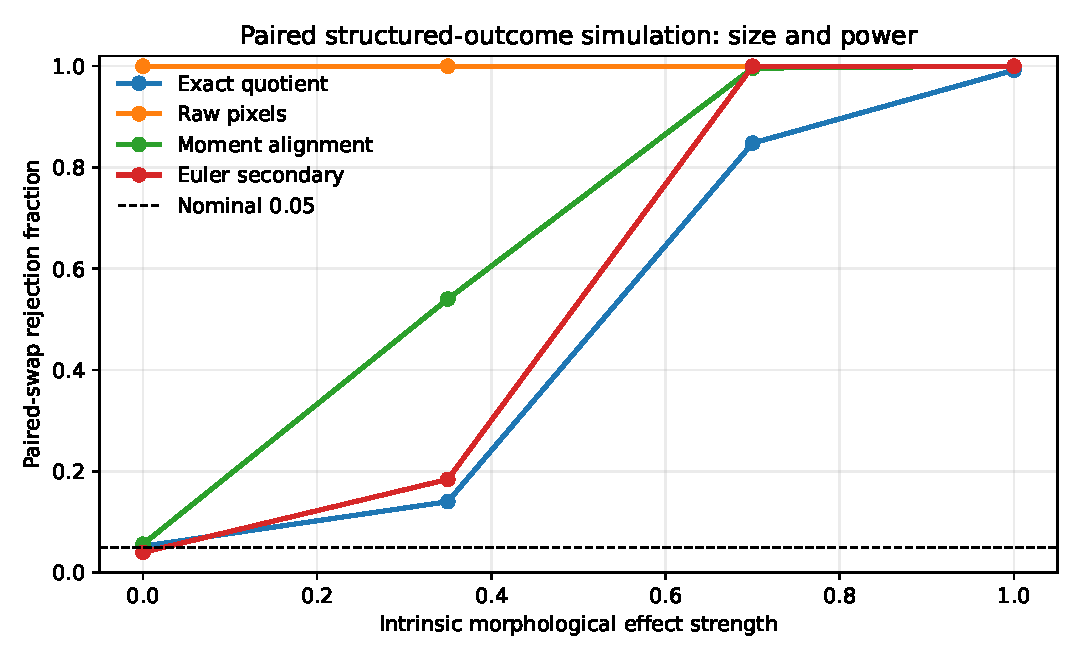
\includegraphics[width=0.78\textwidth]{figures/simulation_power.pdf}
\caption{Paired-swap rejection fractions across intrinsic effect strengths.
Finite-sample causal validity under informative acquisition pertains to the
exact quotient and post-canonical Euler endpoints; raw coordinates and moment
registration are included as diagnostics.}
\label{fig:simulation-power}
\end{figure}

The null column in \cref{tab:simulation} is a Monte Carlo evaluation of the
complete randomization pipeline.  For the exact quotient and post-canonical
Euler tests, the positive-\(\eta\) columns estimate power against a known
intrinsic morphological effect.  For the raw-coordinate and
moment-registration diagnostics they are rejection fractions only, because
those procedures do not have the invariant-endpoint validity guarantee of
\cref{thm:randomization} under informative acquisition.
\else
\paragraph{Analysis status.}
The simulation design and analysis code are frozen, but no numerical simulation
result is reported until the run completes and the generated results file marks
the analysis as available.
\fi

\section{RxRx1 confirmation experiment}

\subsection{Experimental units and frozen selection}

The public RxRx1 release contains 125,510 six-channel \(512\times512\)
fluorescence microscopy images, with two nonoverlapping sites per well, 51
experimental batches, four cell types, and 1,138 siRNAs including 1,108
noncontrol perturbations \citep{sypetkowski2023rxrx1,rxrx1website}.  HUVEC
contributes 24 batches.  The experimental unit in our analysis is the well;
sites and pixels are never treated as independent replicates.  The causal
conditions are the applied siRNA reagents, so the estimand is a
reagent-condition contrast rather than a gene-specific biological effect.

RxRx1 partitions the 1,108 treatment siRNAs into four groups of 277 that
remain together on a plate, and its documentation reports that their well
locations were randomized within experiment and plate
\citep{sypetkowski2023rxrx1}.  A paired randomization analysis must
therefore compare conditions in the same group.  We use HUVEC-01 through
HUVEC-12 as \(\RxDiscoveryBatches\) discovery batches, reserve HUVEC-13 through
HUVEC-16, and use the image rows from HUVEC-17 through HUVEC-24 as
\(\RxConfirmationBatches\) confirmation batches.

Selection uses the public 128-dimensional RxRx1 embeddings in discovery only.
The two site embeddings are averaged within well, and each coordinate is
median-centered and scaled by \(1.4826\) times its median absolute deviation
over all noncontrol treatment wells within that discovery batch; any resulting
scale below \(10^{-6}\) is replaced by \(1\).  Write \(E_{je}\in\bR^{128}\) for the normalized
embedding of condition \(j\) in experiment \(e\).  Split the discovery batches
into \(H_1=\{1,\ldots,6\}\) and \(H_2=\{7,\ldots,12\}\), and define
\[
\begin{aligned}
 \bar E_{jh}&=|H_h|^{-1}\sum_{e\in H_h}E_{je},&
 V_{jh}&=|H_h|^{-1}\sum_{e\in H_h}
          \|E_{je}-\bar E_{jh}\|_2^2,\\
 \delta_h(j,k)&=\bar E_{jh}-\bar E_{kh},&
 R_h(j,k)&=\frac{\|\delta_h(j,k)\|_2^2}
 {V_{jh}+V_{kh}+10^{-12}} .
\end{aligned}
\]
For a pair \((j,k)\), its stability score is
\begin{equation}\label{eq:selection-score}
 S(j,k)=
 \min_{h\in\{1,2\}}R_h(j,k)
 \max\left\{
 \frac{\langle\delta_1(j,k),\delta_2(j,k)\rangle}
 {\sqrt{(\|\delta_1(j,k)\|_2^2+10^{-12})
        (\|\delta_2(j,k)\|_2^2+10^{-12})}},
 0\right\}.
\end{equation}
Eligibility requires exactly one two-site well for each condition in every
discovery batch and an identical discovery-batch plate signature for the two
conditions.  Candidates are ordered by \(S(j,k)\), then by descending minimum
half-SNR, direction cosine, and mean half-SNR, followed by ascending integer
identifiers; greedy matching gives
\(\RxSelectedPairs\) disjoint pairs.  The \(S\)-highest pair is primary and the
remaining \(\RxReplicationPairs\) form a secondary-contrast panel.
Neither confirmation metadata, confirmation embeddings, nor confirmation
images enter this discovery-only selector.

The public release documents which rows are discovery/train and
confirmation/test, but does not establish that the released embedding
generator itself was trained independently of all confirmation images.
Accordingly, the split certifies row-level exclusion; the assignment-based
interpretation additionally assumes that the frozen condition list is
independent of confirmation assignment outcomes.

The discovery-only selection manifest and its SHA-256 integrity digest are
frozen before confirmation image analysis.  A prior implementation also
filtered on confirmation completeness; a replay that removed every
confirmation field returned exactly the same ten ordered pairs and scores.
The earlier manifest is retained as an invalidated audit record.  Before
analysis, a separate confirmation metadata pass must establish completeness
and same-plate occurrence; failure of either gate terminates the analysis.
The checksum records integrity but is not an externally timestamped
preregistration.  Each eligible contrast has
\(\RxConfirmationBlocks\) paired confirmation blocks and therefore
\(\RxPermutationCount\) assignments in its exact randomization distribution.
The frozen confirmation subset contains 160 wells, 320 sites, and 1,920
single-channel PNG files.

\subsection{Estimator-unobserved acquisition stress test}

Each confirmation site is loaded as six 8-bit channels and embedded as a
finite-support lattice array by \(512\)-to-\(64\) Pillow BOX resampling,
retaining 8-bit values, and then adding a 16-pixel zero border.  The nonzero
support bounding box is therefore in \(\cX_{6,64}\), while the larger
\(96\times96\) storage canvas prevents cropping during the imposed motion.

For the six-channel array \(I_{ws}\) from well \(w\) and site \(s\), define the
coordinate-free morphology score and its pooled median by
\[
 m_{ws}=\operatorname{mean}(I_{ws}/255)
       +0.25\,\operatorname{sd}(I_{ws}/255),
 \qquad
 \widetilde m=\operatorname{median}_{w,s}m_{ws}.
\]
For each published nuisance seed, the UTF-8 string
\(\texttt{seed|well\_id|site=s}\) is hashed to a 24-byte BLAKE2b digest, which
is split consecutively into three little-endian unsigned 64-bit integers
\(H_{0,ws},H_{1,ws},H_{2,ws}\).  With treatment label \(a_w\in\{0,1\}\), put
\[
\begin{aligned}
 b_{ws}&=\1\{m_{ws}>\widetilde m\},&
 q_{ws}&=\left\lfloor 1000003\,|m_{ws}|\right\rfloor,\\
 r_{ws}&=(H_{0,ws}\bmod 2+2a_w+b_{ws})\bmod4,&
 d_w&=2a_w-1,\\
 \Delta y_{ws}
 &=d_w\{1+(H_{1,ws}+q_{ws})\bmod8\},&
 \Delta x_{ws}
 &=d_w\{1+(H_{2,ws}+7q_{ws}+b_{ws})\bmod8\}.
\end{aligned}
\]
All six channels at a site receive the same quarter turn \(r_{ws}\) and
translation \((\Delta x_{ws},\Delta y_{ws})\), while the two sites receive
separate, site-specific transformations.  Thus the nuisance distribution is both
treatment- and outcome-dependent and every realized transformation belongs to
the declared product group.  The realized transformation parameters are
logged separately but are not supplied to any representation or test
routine.  No interpolation is used, and the software aborts if nonzero support
is cropped.

This is a controlled unknown-acquisition experiment on real biological images:
the content and batch structure are those of RxRx1, while the transformation
law is imposed so that nuisance ground truth is available for audit but absent
from estimator inputs.  The claim evaluated is invariance to the declared
lattice rigid-motion action, including when the nuisance is treatment- and
outcome-dependent.

\subsection{Endpoints, controls, and inference}

The confirmatory endpoint is the two-site canonical pixel code
\eqref{eq:well-code}, compared by Gaussian-kernel MMD and the complete
\(2^{\RxConfirmationBlocks}\) paired randomization distribution.  The primary
pair is tested at level \(0.05\).  The same canonical-pixel statistic is then
applied to the \(\RxReplicationPairs\) prespecified secondary contrasts, whose
exact \(p\)-values are adjusted together by Holm's method to control familywise
error at \(0.05\).  For the primary pair, the finite Euler signature is a
secondary invariant summary.  Raw transformed pixels and moment registration
are acquisition-sensitive diagnostics; their paired-swap \(p\)-values are
fully enumerated but do not inherit causal validity under informative
acquisition.  The prespecified analysis also generated
\(\RxBootstrapReplicates\) paired-block bootstrap resamples.  Resampling eight
blocks with replacement duplicates observations; applying the conventional
observation-level U-statistic to those duplicated rows changes its
diagonal-exclusion structure.  The resulting quantiles are therefore retained
as a descriptive audit of the resampled statistic, not as confidence intervals
or precision bounds.  Robustness to the transformation
generator is evaluated over \(\RxNuisanceSeeds\) frozen seeds.  Seed
\(20260731\) is the prespecified primary acquisition realization used for the
primary table, its four bootstrap-statistic quantile pairs, the secondary-contrast panel, and
the approximate-action baseline; the other 19 seeds assess robustness of exact
invariance and acquisition-only behavior.  Software tests
and internal orbit audits are completed before the outcome tables are
generated.

Two controls separate exact group invariance from approximate robustness.
First, for every pair and confirmation block, an acquisition-only sharp-null
prototype is constructed by averaging the two clean well arrays and rounding
back to 8-bit values; the same prototype is assigned to both conditions before
the label-dependent hidden motion is applied.  This guarantees equality of the
intrinsic potential outcomes while retaining informative acquisition.  The
resulting rejection fractions are descriptive stress-test summaries over
pairs and nuisance seeds; the independent simulation provides the formal Monte
Carlo type-I assessment.  Second, the primary pair is perturbed outside the
declared action by interpolated rotations of \(5^\circ\), \(10^\circ\), and
\(20^\circ\), two-pixel support truncation, and within-support Gaussian noise of
standard deviation two.  Changes in features, test statistics, and
\(p\)-values quantify sensitivity when the acquisition process only
approximately follows the action.  Before these perturbations, every site in
the seed-\(20260731\) contaminated primary-pair arrays is support-centered.
For method \(m\), if \(Z_m^{(0)}\) and \(Z_m^{(\delta)}\) are the resulting
baseline and perturbed feature matrices, the reported relative error is
\[
 \varepsilon_m(\delta)=
 \frac{\|Z_m^{(\delta)}-Z_m^{(0)}\|_F}
 {\max\{\|Z_m^{(0)}\|_F,10^{-12}\}}.
\]
The label-free median bandwidth rule is recomputed from the pooled primary-pair
features for every perturbation before its statistic and complete paired-swap
\(p\)-value are evaluated.

\subsection{Results}

\ifresultsavailable
The primary contrast is siRNA 384 (\RxTreatmentA) versus siRNA 747
(\RxTreatmentB).  The confirmation completeness and same-plate gate
\RxPlateAudit.  The discovery-only selection manifest has SHA-256
{\scriptsize\texttt{\RxManifestHash}}.

\begin{table}[htbp]
\centering
\caption{RxRx1 analysis for the primary pair under imposed lattice rigid
motions whose parameters are excluded from estimator inputs.  The displayed
kernel discrepancy is defined in
\eqref{eq:mmd}, and \(p\)-values enumerate all paired label swaps.  The
canonical-pixel endpoint is the sole primary test.  The Euler \(p\)-value is an
unadjusted secondary analysis; raw and moment-registration values are
diagnostics.  The finite-sample causal validity theorem applies to the
invariant quotient and post-canonical Euler rows, not to the raw or
moment-registration diagnostics.}
\label{tab:rxrx}
\begin{tabular}{lcc}
\toprule
Representation & \(\widehat{\MMD}_u^2\) & Paired-swap \(p\)\\
\midrule
Canonical quotient pixels
  & \RxCanonicalMMD & \RxCanonicalP\\
Finite directional Euler signature
  & \RxEulerMMD & \RxEulerP\\
Moment registration
  & \RxMomentMMD & \RxMomentP\\
Raw transformed pixels
  & \RxRawMMD & \RxRawP\\
\bottomrule
\end{tabular}
\end{table}

\begin{table}[htbp]
\centering
\caption{Prespecified paired-block bootstrap audit for the primary contrast.
The last column contains the empirical 2.5th and 97.5th percentiles of the
resampled U-statistic over \(\RxBootstrapReplicates\) draws.  Because duplicate
blocks alter the conventional observation-level U-statistic's
diagonal-exclusion structure at \(B=8\), these quantiles are not confidence
intervals and are not interpreted as uncertainty bounds around the point
statistic.}
\label{tab:rxrx-bootstrap-audit}
\begin{tabular}{lcc}
\toprule
Representation & Original \(\widehat{\MMD}_u^2\)
& Bootstrap-statistic quantiles\\
\midrule
Canonical quotient pixels
  & \RxCanonicalMMD & \RxCanonicalMMDCI\\
Finite directional Euler signature
  & \RxEulerMMD & \RxEulerMMDCI\\
Moment registration
  & \RxMomentMMD & \RxMomentMMDCI\\
Raw transformed pixels
  & \RxRawMMD & \RxRawMMDCI\\
\bottomrule
\end{tabular}
\end{table}

\begin{table}[htbp]
\centering
\caption{Canonical-quotient tests for the prespecified secondary-contrast
panel.  Holm adjustment is applied to the family of
\(\RxReplicationPairs\) secondary-contrast \(p\)-values; these are different
siRNA contrasts, not biological replications of the primary contrast.}
\label{tab:rxrx-replications}
\begin{tabular}{clccc}
\toprule
Pair & Conditions & \(\widehat{\MMD}_u^2\) & Swap \(p\) & Holm \(p\)\\
\midrule
\RxReplicationRows
\bottomrule
\end{tabular}
\end{table}

\RxReplicationSummary

Across all acquisition-transform seeds, the maximum absolute clean-versus-
contaminated feature discrepancies were \(\RxMaxQuotientFeatureError\) for the
maximal-invariant pixels and \(\RxMaxEulerFeatureError\) for the finite Euler
signature.  For the maximal-invariant endpoint, the largest corresponding
changes in \(\widehat{\MMD}_u^2\) and its exact \(p\)-value were
\(\RxMaxQuotientStatisticError\) and \(\RxMaxQuotientPError\), respectively.

\begin{table}[htbp]
\centering
\caption{Acquisition-only sharp-null stress test over frozen pairs and hidden
nuisance seeds.  The intrinsic array is identical for both conditions within
each block before the treatment-dependent acquisition motion.}
\label{tab:acquisition-null}
\begin{tabular}{lccc}
\toprule
Method & Tests & Rejections at 0.05 & Rejection fraction\\
\midrule
\RxAcquisitionNullRows
\bottomrule
\end{tabular}
\end{table}

\begin{table}[htbp]
\centering
\caption{Approximate-action stress test for the primary pair.  Feature error is
relative to the exactly transformed baseline; the last two columns give
absolute changes from the baseline statistic and exact \(p\)-value.}
\label{tab:approximate-action}
\resizebox{\textwidth}{!}{%
\begin{tabular}{llccc}
\toprule
Perturbation & Method & Relative feature error
& \(\lvert\Delta\widehat{\MMD}_u^2\rvert\)
& \(\lvert\Delta p\rvert\)\\
\midrule
\RxApproximateStressRows
\bottomrule
\end{tabular}
}
\end{table}

\ifextensionsavailable
\subsection{Post-analysis sensitivity and persistence diagnostics}

The following two diagnostics were specified after the confirmatory outcomes
and primary result had been accessed.  They neither alter the frozen endpoint
nor convert the extension into a confirmatory analysis.  First, we evaluated
\cref{prop:sensitivity} for the primary canonical-quotient statistic.  The
calculation enumerated all 256 assignments and all 256 vertices of the
bounded-odds probability box at each value of \(\Lambda\).  The machine-readable
extension audit has SHA-256
{\scriptsize\texttt{\RxExtensionAuditHash}}.

\begin{table}[htbp]
\centering
\caption{Post-analysis sensitivity of the primary quotient test to departure
from uniform paired assignment.  The second column is the exact worst-case
upper-tail probability under the independent product model in
\eqref{eq:sensitivity-model}.}
\label{tab:sensitivity}
\begin{tabular}{cc}
\toprule
Sensitivity factor \(\Lambda\) & Worst-case upper \(p\)\\
\midrule
\RxSensitivityRows
\bottomrule
\end{tabular}
\end{table}

At \(\Lambda=1\), the envelope reproduces the complete paired-swap value
\(\RxExtensionExactP\).  The worst-case upper probability first reaches 0.05
at \(\Lambda=\RxSensitivityCritical\) (numerical upper probability
\(\RxSensitivityCriticalP\)).  Thus, within the conditional-independence model
\eqref{eq:sensitivity-model}, the primary conclusion remains below 0.05 for
smaller sensitivity factors.  This statement quantifies possible
nonuniformity of the reported assignment mechanism; it is not an estimate of a
specific unmeasured confounder's effect.

Second, we evaluated a lower-star, zero-dimensional persistence diagnostic on
the 16-by-16 resampled invariant nuclear-channel representation for all
\(\RxPersistenceSites\) primary-pair sites.  All
\(\RxPersistenceInvariantChecks\) diagrams were exactly invariant under the
recorded hidden lattice actions, with maximum bottleneck distance
\(\RxPersistenceMaxExactBottleneck\).  After an independently generated
one-gray-level bounded perturbation, all \(\RxPersistenceStabilityChecks\)
diagram comparisons satisfied the bottleneck stability inequality and all
\(\RxPersistenceKernelChecks\) diagnostic-Gaussian-metric inversion checks
passed.  The
largest bottleneck distance was \(\RxPersistenceMaxPerturbedBottleneck\), no
larger than the largest realized sup-norm perturbation
\(\RxPersistenceMaxSupNorm\).  This audit concerns the stable grayscale
filtration in \cref{thm:persistence-kernel}, not the thresholded finite Euler
signature.
\else
\paragraph{Extension status.}
No bounded-odds or stable-persistence numerical result is reported until the
post-analysis extension runner completes and its audited TeX file is present.
\fi

The internal algebraic and software audit recorded
\(\RxInvariantAuditFailures\) canonical-code failures among
\(\RxInvariantAuditTrials\) generated transformations.  The software test suite
passed \(\SoftwareTestsPassed\) checks.  Its source fingerprint is
\texttt{\SoftwareCommit}.
\else
\paragraph{Analysis status.}
The discovery rule and analysis code are frozen.  No RxRx1 outcome estimate,
\(p\)-value, audit result, or secondary-contrast claim is reported until the
confirmation run completes and the generated results file marks the analysis
as available.
\fi

\FloatBarrier
\section{Discussion}

The observation model \eqref{eq:observation-model} permits a particularly
adversarial nuisance: acquisition may depend on both treatment and outcome.
Under that model, \cref{thm:sharp} gives a sharp boundary.  An invariant target
is observed exactly; a noninvariant target cannot be recovered uniformly
without additional information.  A maximal invariant reaches this boundary by
retaining the full orbit.  Causal identification remains a separate step,
supplied here either by quotient-specific exchangeability in
\cref{thm:gformula} or by the randomization design under the conditional
uniformity premise motivated by the reported within-plate randomization in
\cref{thm:randomization}.

The lattice construction also shows that compactness is not necessary when an
explicit measurable cross-section is available.  Integer translations form a
noncompact group, yet support normalization followed by finite rotational
canonicalization is exact and maximal.  This avoids a nuisance-distribution
model and preserves every feature that is identifiable modulo the declared
rigid motions.  The Gaussian quotient kernel is characteristic for quotient
laws and supplies the discrepancy statistic used in the sharp-null test,
whereas the finite Euler vector answers a deliberately lower-dimensional
secondary question.

The padding and support checks in the controlled experiment ensure that the
imposed translations preserve the full nonzero support.  If a natural field of
view clips that support, the appropriate model is
\(X=\Pi\{\Gamma\cdot Y(A)\}\), and \cref{thm:partial-observation} replaces
ordinary orbit invariance.  In particular, if two distinct intrinsic orbits
can produce the same crop, their maximal-orbit label is not recoverable from
that crop.  The support-truncation stressor removes a margin from the realized
support bounding box; it demonstrates sensitivity to loss of intrinsic content
but is not a simulation of translation through a fixed sensor boundary and
does not restore identification.

Abstract continuous rotations are covered by \cref{cor:continuous-rotations};
the unresolved computational issue is an exact, useful representation for the
chosen continuous action.  On a pixel lattice, interpolated rotation is not the
same operation as the exact \(C_4\) permutation used here.  Similarly,
\cref{cor:invariant-cate} identifies conditional effects only after an
integrable scalar invariant functional and adequate covariates are specified.
With eight primary blocks and no prespecified subgroup model, fitting a
high-dimensional heterogeneous-effect learner would not support credible
inference, so none is reported.

The scientific interpretation is action-specific.  The empirical intervention
validates the method against imposed integer translations and quarter turns
whose realized elements are excluded from estimator inputs;
it does not convert general optical deformation, rescaling, or changing cell
content into members of that action.  Likewise, inference from the reported
RxRx1 within-plate randomization concerns the selected siRNA reagents in the
analyzed HUVEC plate design.
These qualifications delimit the estimand rather than weaken identification:
within the stated action, invariance is algebraic; under the conditional
uniformity, no-interference, well-defined-version, and swap-invariant-retention
assumptions, randomization validity is finite-sample exact for the invariant
Fisher sharp null.

\section{Conclusion}

Unknown unit-specific transformations need not be estimated in order to conduct
causal inference on the information that survives them.  For measurable group
contamination, orbit invariance is necessary and sufficient for exact
observability, and a Borel maximal invariant carries every such target.  We
provide a complete identification formula for its interventional law, an
explicit maximal invariant for multichannel lattice images under
\(\bZ^2\rtimes C_4\), and an exact paired randomization test using a
characteristic quotient kernel.  The simulation and RxRx1
discovery--confirmation experiments turn these population statements into an
auditable workflow with informative acquisition transformations whose realized
parameters are excluded from estimator inputs.

\section*{Reproducibility statement}

The accompanying software downloads the frozen RxRx1 subset, verifies file and
manifest hashes, displays progress for data acquisition and every simulation
stage, constructs all four representations, enumerates the complete assignment
distribution, computes bootstrap and multiplicity-adjusted summaries, executes
the unit tests, and writes the numerical macros consumed by this manuscript.
The analysis uses only public RxRx1 data subject to its stated license
\citep{rxrx1website}.

\bibliographystyle{plainnat}
\bibliography{references}

\end{document}
